\subsection{Overall accuracy of  the simplified Ikeda method}
\label{se:overall_comparison}
Comparing roll damping is a bit difficult since the roll damping model consist of two coefficients: a linear term $B_1$ and a quadratic term $B_2$. These coefficients can however be combined by calculating the equivalent damping coefficient for a certain roll angle $\phi_a$ \parencite{himeno_prediction_1981}:

\begin{equation}
B_{e} = B_{1} + \frac{8 B_{2} \omega_{0} \phi_{a}}{3 \pi}
\end{equation}


For the roll damping database $B_1$ and $B_2$ can be inserted directly into Eq.(\ref{eq:B_e_equation}) to get the equivalent roll damping $B_e$. In order to obtain the same coefficients for the SI-method, roll damping was calculated for two roll amplitudes $\phi_a$ for the same motion frequency. $B_1$ and $B_2$ are obtained by fitting Eq.(\ref{eq:B_e_equation}) to this data \parencite{himeno_prediction_1981}. The $B_e$ coefficient was made non-dimensional according to \parencite{himeno_prediction_1981},  giving the non-dimensional equivalent linear damping coefficient $\hat{B_e}$, which was more convenient to use for this comparison as follows,
\begin{equation} \label{eq:be_eqvalent}
    \hat{B_e} = \frac{B_e}{\rho \bigtriangledown Beam^2} \sqrt{\frac{Beam}{2g}},
\end{equation}
where $\rho$, $\bigtriangledown$ and $Beam$ stand for fluid density, displacement volume, and breadth of a ship, respectively.
For the roll decay tests at SSPA, i.e., the database used in this study, the initial roll angle is normally set to 10 degrees, so that the model test data contain amplitudes in the range from 0 to 10 degrees. The root mean squared error of the equivalent roll damping, $RMSE_{\hat{B}_e}$, for various initial roll angles $\hat{B}_e(\phi_a)$ between estimations using the SI-method and the model test results is,

\begin{equation} \label{eq:rmse}
    RMSE({\hat{B}_e} (\phi_a)) = \sqrt{\frac{\sum\limits_{i=1}^n (\hat{B}_{e,i}^{SI} (\phi_a) - \hat{B}_{e,i}^{model} (\phi_a))^2}{n}},
\end{equation}
where $\hat{B}_{e,i}^{SI} (\phi_a)$ represents the equivalent roll damping by the SI-method for the \emph{i}th model test with initial roll angle of $\phi_a$, while $\hat{B}_{e,i}^{model} (\phi_a)$ represents the damping from the model tests. The results of the RMSE are plotted in the upper plot of Fig.\ref{fig:ikeda_phi_a}. Large values of $RMSE({\hat{B}_e})$ indicate very bad agreement between the SI-method and the model test results for roll damping prediction of modern ships. It should be noted that the accuracy decreases for larger amplitudes where the nonlinear portion of the SI-method plays a larger role. Furthermore, in order to illustrate the difference of $\hat{B}_e$ prediction between the SI-method and the model tests at SSPA, the three bottom plots of Fig.\ref{fig:ikeda_phi_a} presents the comparison for three roll amplitudes $\phi_a$ equal to 0, 5, and 10 degrees, respectively. This shows that accuracy differs greatly between the amplitudes, with the highest accuracy at zero roll amplitude, and it raises the question at what roll amplitude should a comparison be conducted? Should the methods be compared at small or large roll amplitudes? In order to avoid this decision, $\hat{B}_e$ is instead calculated for a range of roll amplitudes (1,2,..10 degrees).   

\begin{figure}[H]
\centering
  \centering
  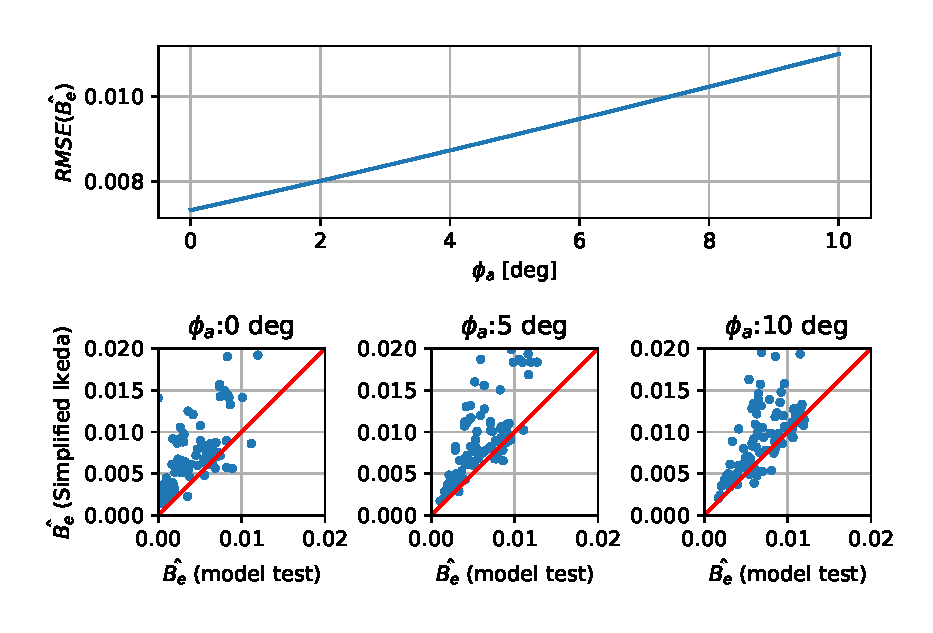
\includegraphics[]{figures/ikeda_phi_a.eps}
  \vspace{-0.5cm}
  \caption{Root mean square error of roll damping prediction between the SI-method and the model test results (upper plot). Influence of roll amplitude $\phi_a$ on $\hat{B_e}$ between the SI-method and model tests for $0^{\circ}$ (bottom left plot), $5^{\circ}$ (bottom middle plot) and $10^{\circ}$ (bottom right plot), respectively.}
  \label{fig:ikeda_phi_a}
\end{figure}

It was found that most of the ships in the roll damping database were outside the limits suitable to be applied in Eq.(\ref{eq:SI_limits}). Fig.\ref{fig:si_model_within} shows the SI-method versus all model tests and versus model tests within the limits. The values of non-dimensional equivalent linear damping $B_e$ for roll amplitudes in the range 0 to 10 degrees are displayed. The points within the limits seem to agree much better with the model tests than the points outside the limits (which are far away from the red reference line). Corresponding $R^2$ are shown in Table \ref{tab:si_validation}. The damping components are plotted against the error in figure \ref{fig:component_residual}, where it looks like the wave damping $B_W$ is very large when the error is large. 


\begin{table}[H]
    \centering
    \caption{Validation of SI within and outside limits}
   \begin{tabular}{lrr}
\toprule
{} &  $R^2$ &  Number of points \\
\midrule
SI no limits     & -46.35 &              1470 \\
SI within limits &   0.83 &               120 \\
\bottomrule
\end{tabular}

    \label{tab:si_validation}
\end{table}
    

\begin{figure}[H]
    \centering
    \begin{subfigure}[b]{0.48\textwidth}
        \centering
  
        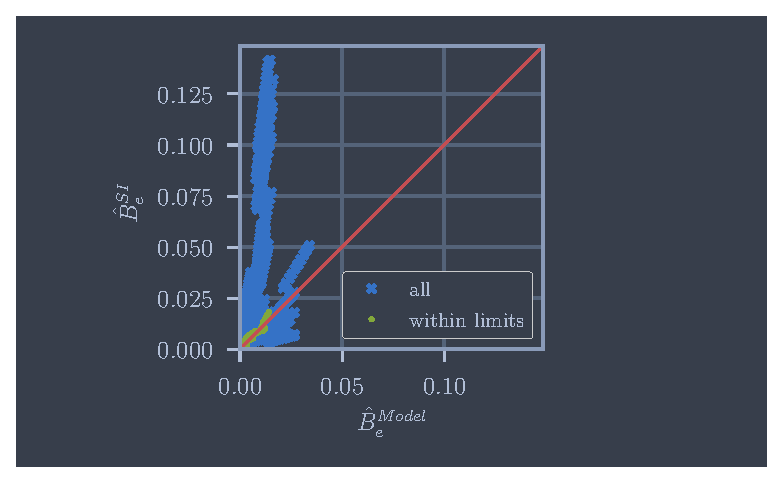
\includegraphics[width=\textwidth]{figures/si_model_within.eps}
        \vspace{-0.5cm}
        \caption{Equivalent linearized damping}
        \label{fig:si_model_within}
    \end{subfigure}
        ~ %add desired spacing between images, e. g. ~, \quad, \qquad, \hfill etc. 
      %(or a blank line to force the subfigure onto a new line)
    \begin{subfigure}[b]{0.48\textwidth}
        \centering
        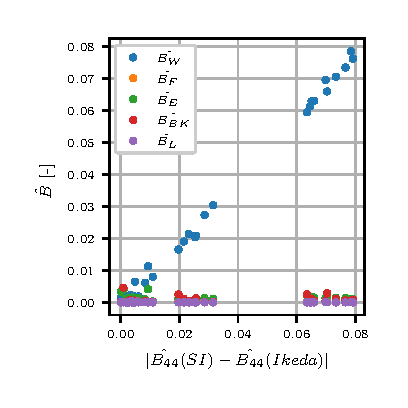
\includegraphics[width=\textwidth]{figures/component_residual.eps}
        \caption{Residual vs. components}
        \label{fig:component_residual}
    \end{subfigure}
    \caption{SI-method with and outside limits vs. model tests}
    
\end{figure}



